\documentclass[12pt]{article}
\usepackage{graphicx}
\usepackage[section]{placeins}
\usepackage{amsmath}
\usepackage{listings}
\usepackage{xcolor}

\usepackage[top=1.0in, bottom=1.0in, left=0.5in, right=0.5in]{geometry}
\renewcommand{\thesection}{}
\renewcommand{\thesubsection}{\arabic{subsection}}
\lstdefinelanguage{VHDL}{
  morekeywords={
    library,use,all,entity,is,port,in,out,end,architecture,of,
    begin,and,case,when,process,ALL,downto,Port,null,others,xor,not,or,map,signal,
    component,if,then,ns,ps,PS,NS,type,constant,time
  },
  morekeywords=[2]{
    STD_LOGIC_VECTOR,STD_LOGIC,IEEE,STD_LOGIC_1164,
    NUMERIC_STD,STD_LOGIC_ARITH,STD_LOGIC_UNSIGNED,std_logic_vector,
    std_logic,std_logic_unsigned,ieee,rising_edge
  },
  morecomment=[l]--
}
\colorlet{keyword}{blue!100!black!80}
\colorlet{comment}{green!90!black!100}
\colorlet{STD}{red!100!white!80}
\colorlet{background}{white!100!black!100}
\lstdefinestyle{vhdl}{
  language     = VHDL,
  basicstyle   = \ttfamily,
  keywordstyle = [1]\color{keyword}\bfseries,
  keywordstyle = [2]\color{STD}\bfseries,
  commentstyle = \color{comment},
}
\lstset{
	frame = single,
	backgroundcolor = \color{background},
	numbers = left,
	captionpos = b,
	stringstyle = \ttfamily\color{red!50!brown}
}

\begin{document}
\title{\vspace{15ex}\Huge{CS 288: Digital Stop Watch}\vspace{15ex}}


\author{
  Dheerendra Singh Rathor\\120050033\\
  \texttt{dheeru.rathor14@gmail.com}\\[1 cm]
}

\date{\today}
\maketitle
\newpage

\section{Aim:}
Using Xilinx ISE design and simulate a digital stop watch module to count in milliseconds.
\begin{itemize}
\item Use 1 KHz as primary clock in design.
\item Module will have three inputs – Start, Stop and Reset to control the stop watch.
\item Use an 8-bit counter for milliseconds count.
\end{itemize}

\section{Procedure:}
For designing a stop watch - I used the following pointers:
\begin{itemize}
\item defined 3 input variable viz start, stop and reset and a clock variable clock and an 8 bit output variable named output.
\item defined clock period as 1 ms
\item defined a state machine with 3 states viz s0, s1 and s2
\item initialized PS and NS as s0
\item defined a clock process for the clock variable with at every rising edge PS is changing to NS and other state changes are simulated with the different input conditions.
\end{itemize}

States are defined as follows:
\begin{itemize}
\item s0: s0 is the initial state where counter is "00000000" and counter will not increase
\item s1: s1 is the counting state. When the state is s1, counter will increase by 1 after every 1 ms
\item s2: s2 is the stopped state. At this state counter will poses a value but will not increase until start is triggered
\end{itemize}

\begin{center}
\begin{tabular}{| l | l | l | l | }
\hline
 Present State & NS at start & NS at stop & NS at reset\\ \hline
 s0 & s1 & s0 & s0 \\ \hline
 s1 & s1 & s2 & s0 \\ \hline
 s2 & s1 & s2 & s0 \\ \hline
\end{tabular}
\end{center}
\newpage
\section{Timing Diagrams}
\begin{figure}[!ht]
\centering
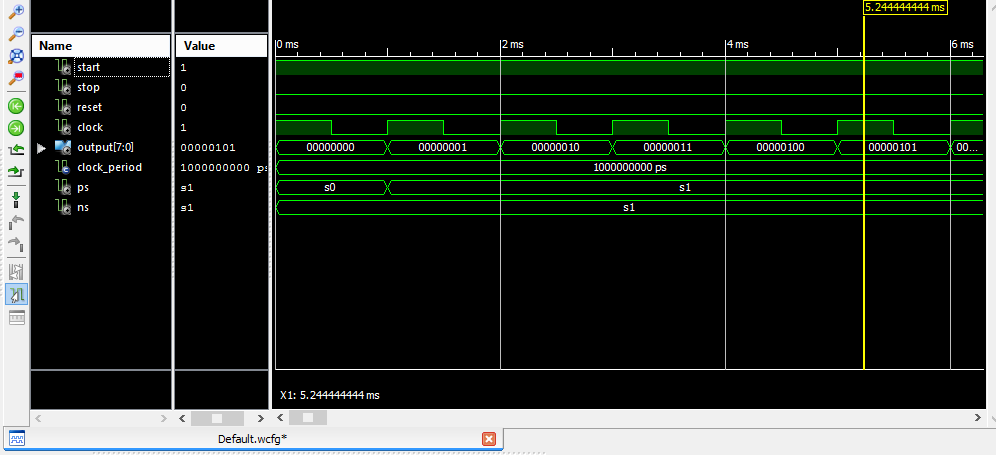
\includegraphics[width=1\textwidth]{Capture}
\caption{Timing diagram showing the increment in counter when the state of the machine is s1}
\label{fig1}
\end{figure}

\begin{figure}
\centering
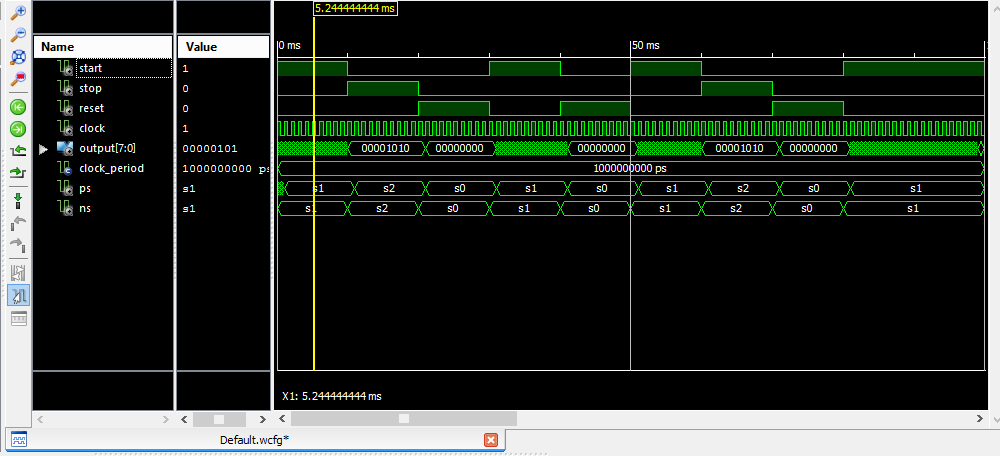
\includegraphics[width=1\textwidth]{Capture1}
\caption{Timing diagram showing the changes in states with change in input}
\label{fig2}
\end{figure}

\begin{figure}
\centering
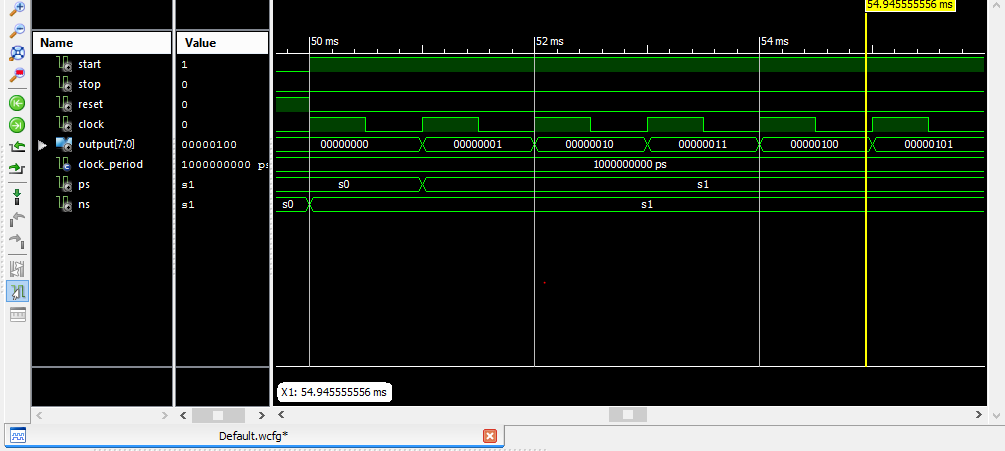
\includegraphics[width=1\textwidth]{Capture2}
\caption{Timing diagram showing the change in output and change in states with the change in input}
\label{fig3}
\end{figure}

\section{Codes}
Here I have include working code for Arithmetic Logic Unit and 4-bit Adder.
\subsection{8 bit milliseconds counter}
\begin{lstlisting}[style=vhdl]
----------------------------------------------------------------------------------
-- Company: 
-- Engineer: 
-- 
-- Create Date:    15:02:32 03/11/2014 
-- Design Name: 
-- Module Name:    main - Behavioral 
-- Project Name: 
-- Target Devices: 
-- Tool versions: 
-- Description: 
--
-- Dependencies: 
--
-- Revision: 
-- Revision 0.01 - File Created
-- Additional Comments: 
--
----------------------------------------------------------------------------------
library IEEE;
use IEEE.STD_LOGIC_1164.ALL;
use ieee.std_logic_unsigned.all;

-- Uncomment the following library declaration if using
-- arithmetic functions with Signed or Unsigned values
--use IEEE.NUMERIC_STD.ALL;

-- Uncomment the following library declaration if instantiating
-- any Xilinx primitives in this code.
--library UNISIM;
--use UNISIM.VComponents.all;

entity main is
    Port ( start : in  STD_LOGIC;
           stop : in  STD_LOGIC;
           reset : in  STD_LOGIC;
           clock : in  STD_LOGIC;
           output : out  STD_LOGIC_VECTOR (7 downto 0));
end main;

architecture Behavioral of main is
constant clock_period : time := 1 ms;
--variable cnt : INTEGER := '0';
type state_type is (s0,s1,s2);
signal ps,ns : state_type:=s0;
signal temp : std_logic_vector (7 downto 0) := "00000000";
--begin process (start,stop,reset)
begin


SEQ:process(clock)
begin
	if (rising_edge(clock)) then
		ps <= ns;
		case ps is 
			when s0 =>
				if (start = '1') then 
					temp <= temp + "00000001";
					output <= temp;
					ns <= s1;
				end if;
				if (stop = '1') then 
					output <= temp;
					ns <= ps;
				end if;
				if (reset = '1') then
					output <= temp;
					ns <= ps;
				end if;
			when s1 => 
				if (start = '1') then 
					temp <= temp + "00000001";
					output <= temp;
					ns <= ps;
				end if;
				if (stop = '1') then 
					output <= temp;
					ns <= s2;
				end if;
				if (reset = '1') then 
					temp <= "00000000";
					output <= temp;
					ns <= s0;
				end if;
			when s2 =>
				if (start = '1') then 
					temp <= temp + "00000001";
					output <= temp;
					ns <= s1;
				end if;
				if (stop = '1') then 
					output <= temp;
					ns <= ps;
				end if;
				if (reset = '1') then 
					temp <= "00000000";
					output <= temp;
					ns <= s0;
				end if;
			when others =>
				null;
		end case;
	end if;
end process;

end Behavioral;


\end{lstlisting}

\section{Inference}
In this assignment I inferred the following:\\
\verb|1.| Working of the clock with different frequencies in VHDL\\
\verb|2.| Learned about using and simulating state machines in VHDL  \\
\verb|3.| Learned using the library \textcolor{STD}{ieee.std\_logic\_unsigned}.\textcolor{keyword}{all}\\
\verb|4.| Representing State Diagrams in VHDL \\
\end{document}
